
\subsection{Approximating an Optimal Path}\label{sec:LP}
In this section an approach to finding a global optimal solution to the optimisation problem proposed in Section \ref{sec:optiprob} is formulated. The optimisation problem is a non-linear optimisation problem, due to the two unknown variables of the objective function \( D(e_i)/v_{e_i} \) and $R_{CO}(v_{e_i})$ being non-linear functions. However, these functions can be used in a linear programming problem by formulating \( D(e_i)/v_{e_i} \) and $R_{CO}(v_{e_i})$ as piece-wise linear functions \cite{ahuja1995capacity}. Specifically, the problem is modelled as a mixed integer problem (MIP) problem. This section introduces the extra constraints necessary to solve the problem as a MIP problem and thereby end up at an approximating optimal solution \cite{piecewiseglpk}. The quality of the solution depends on how many pieces the non-linear function is split into. \todo[inline]{Explain that this problem is in NP}

The linearization of a function is handled as shown in Figure \ref{fig:linearization_example}. The non-linear function is split into a number of linear pieces. To handle the linearization three new sets are introduced, a set of known variables which is the pre computed function of each linear piece, and another set of known variables which is the start and end points of each line segment and a set of unknown variables which will be the line segment chosen. The unknown variable is called selected line (SL) which have a two dimensional size $n \times m$ where $n$ is the amount of edges with a unique function. $m$ is the number of linear lines every edge's function is split into. This leads to the following constraints:  

\begin{figure}[h!]
\centering
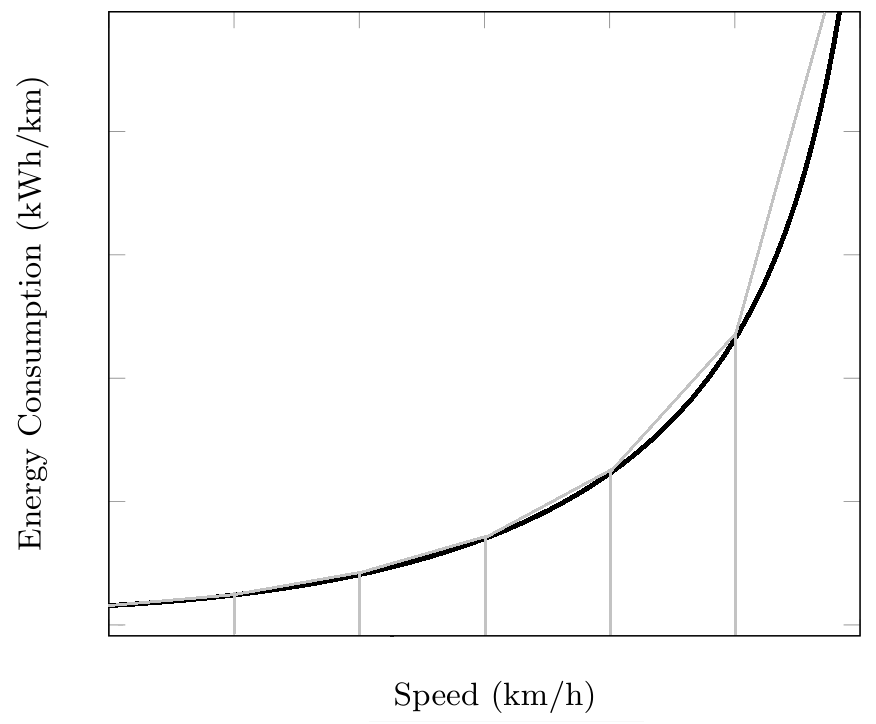
\includegraphics[scale=0.33]{images/linearization_example}
\caption{Example of a non-linear function which is split into 6 pieces}
\label{fig:linearization_example}
\end{figure}

For n edges, exactly n line segments needs to be selected. In other words, for every edge, only one linear line is chosen. 
\begin{equation*}
\forall_{i\in1 \dots n }:\; \sum_{j=1}^{m} SL_{i,j} = 1
\end{equation*}
$n$ is the length of the path, $m$ is the amount of lines the functions \( D(e_i)/v_{e_i} \) and $R_{CO}(v_{e_i})$ are split into and $\sum_{j=1}^{m} SL_{i,j} = 1$ ensures that only one line segments can be selected, because exactly one line segment needs to be chosen. In other words, SL needs to be binary values.
\begin{equation*}
\forall_{i\in1 \dots n, j \in 1 \dots m}: \; \; SL_{i,j} \in{0,1} 
\end{equation*}
The speed of the EV needs to be constrained by the line segment chosen:
\begin{equation*}
\forall_{i\in1 \dots n, j \in 1 \dots m-1}:\; SL_{i,j} * P_{i,j}  \le  v_{j,e_i} \le SL_{i,j}*P_{i,j+1}
\end{equation*}
$P$ is the set of starting points of all line segments including the end point of the previous segment. $SL_{i,j} * P_{i,j}$ is the minimal speed the EV is allowed to drive on edge $i$ and $SL_{i,j}*P_{i,j+1}$ is the maximal speed, note that the values will either be a valid value or $0$, if the segment is not selected being that $SL_{i,j}$ is $0$ if the line segment is not chosen. $P_{i,j+1}$ is the end point of $P_{i,j}$. 
The linearization of \( D(e_i)/v_{e_i} \) and $R_{CO}(v_{e_i})$ can now be found by pre-computing the line segments of each of the path edges. for instance, to linearize $R_{CO}(v_{e_i})$ we pre-compute a set of line functions on the form $a*x+b$. We store the slope $a$ as $Slopes$, and the constants $b$ as $Constants$. In total $n \times m$ function are defined. The linearized model of $R_{CO}(v_{e_i})$ for every edge $i$ will look like this:
\begin{equation*}
\sum_{j=1}^{m} Slopes_{i,j}*v_{e_i,j} + \sum_{j=1}^{m} SL_{i,j}*Constants_{i,j} 
\end{equation*}
\todo[inline]{Explicitly explain what $v_{e_i,j}$ is}
$\sum_{j=1}^{m} Slopes_{i,j}*v_{e_i,j}$ is equivalent of $a*x$ and $\sum_{j=1}^{m} SL_{i,j}*Constants_{i,j}$ is equivalent with $b$ and thus the consumption rate of the EV is modelled as $m$ functions. 
Finally note that this is a way to determine the solution of $R_{CO}(v_{e_i})$ and before a solution to an edge can be found, the line segments and points for both of the non linear functions needs to be pre-computed. 
%sources
%1, SWP-3587
%2, glpk-sos2
